\documentclass{wrcreport}

\ifx\pdftexversion\undefined
\usepackage[dvips]{graphicx}
\else
\usepackage[pdftex]{graphicx}
% Only print picture outlines...
%\usepackage[pdftex,draft]{graphicx}
\DeclareGraphicsRule{*}{mps}{*}{}
\fi

\usepackage{siunitx}
\usepackage{minitoc}
\usepackage{pdfpages}

%\usepackage[a4paper,lmargin=3.0cm, rmargin=1.0cm,tmargin=3.5cm,bmargin=2.50cm]{geometry}

%%%%%%%%%%%%%%%%%%%%%%%%%%%%%%%%%%%%%%%%%%%%%%%%%%%%%%%
% Reset text/figure fractions to more reasonable values
%%%%%%%%%%%%%%%%%%%%%%%%%%%%%%%%%%%%%%%%%%%%%%%%%%%%%%%
\renewcommand{\topfraction}{0.85}
\renewcommand{\textfraction}{0.1}
\renewcommand{\floatpagefraction}{0.79}
%%%%%%%%%%%%%%%%%%%%%%%%%%%%%%%%%%%%%%%%%%%%%%%%%%%%%%%
% Working
%\renewcommand{\topfraction}{0.85}
%\renewcommand{\textfraction}{0.}
%\renewcommand{\floatpagefraction}{0.79}
%%%%%%%%%%%%%%%%%%%%%%%%%%%%%%%%%%%%%%%%%%%%%%%%%%%%%%%

\graphicspath{{./images/}}

\usepackage{longtable}
%\usepackage{fullpage} % reduce margin whitespace
%\usepackage{setspace} % 

% This makes TOC and lists have very little white spacing...
\usepackage{tocloft}
%%%%%%%%%%%%%%%%%%%%%%%%%%%%%%%%%%%%%%%%%%%%%%%%%%%%%%%
% Draft assistance
%%%%%%%%%%%%%%%%%%%%%%%%%%%%%%%%%%%%%%%%%%%%%%%%%%%%%%%
%\usepackage{showkeys}
%\usepackage{showlabels}
%\usepackage{everypage}
%\usepackage{draftwatermark}
%%%%%%%%%%%%%%%%%%%%%%%%%%%%%%%%%%%%%%%%%%%%%%%%%%%%%%%

\usepackage{times} % font
\usepackage{booktabs}
\usepackage{multirow}
\usepackage{cmap}     % to produce searchable PDF
\usepackage{rotating,lscape}

%%%%%%%%%%%%%%%%%%%%%%%%%%%%%%%%%%%%%%%%%%%%%%%%%%%%%%%
% Page style - footers and headers
%%%%%%%%%%%%%%%%%%%%%%%%%%%%%%%%%%%%%%%%%%%%%%%%%%%%%%%
\usepackage{fancyhdr}

\pagestyle{fancy}
\renewcommand{\chaptermark}[1]{\markboth{\thechapter.\ #1}{}} 
\fancyhead{} % clear all header fields

\fancypagestyle{plain}{%
  \renewcommand{\headrulewidth}{0pt}% Header rule thickness
  \renewcommand{\footrulewidth}{0pt}% Footer rule thickness
  \fancyhf{}% Clear header/footer
  \renewcommand{\headrulewidth}{\iffloatpage{0pt}{0pt}}
  \fancyfoot[C]{-\thepage-} % Page number at the bottom 
}
%\fancypagestyle{frontmatter}{%
%  \renewcommand{\headrulewidth}{0pt}% No header rule
%  \renewcommand{\footrulewidth}{0pt}% No footer rule
%  \fancyhf{}% Clear header/footer
%  \fancyfoot[C]{-\thepage-}%
%}
\fancypagestyle{mainmatter}{%
  \renewcommand{\headrulewidth}{0pt}% Header rule
  \renewcommand{\footrulewidth}{0pt}% Footer rule
  \fancyhf{}% Clear header/footer
  \fancyhead[L]{\scshape\leftmark}% Chapter in header Left
  \fancyhead[R]{WRC Progress Report K5 Number: 2062}% Page number in header Right
  \renewcommand{\headrulewidth}{\iffloatpage{0pt}{0pt}}
  \fancyfoot[C]{-\thepage-} % Page number at the bottom 
}

%%%%%%%%%%%%%%%%%%%%%%%%%%%%%%%%%%%%%%%%%%%%%%%%%%%%%%%

\usepackage[section]{placeins}
\usepackage{amsmath,url}
\usepackage{subeqnarray}

%pdfpagelabels, % Need to solve the figure count reset to use this

%%%%%%%%%%%%%%%%%%%%%%%%%%%%%%%%%%%%%%%%%%%%%%%%%%%%%%%%%%%%%
% Hyperref pdf options
%%%%%%%%%%%%%%%%%%%%%%%%%%%%%%%%%%%%%%%%%%%%%%%%%%%%%%%%%%%%%
\usepackage[pdftitle={Quantifying rainfall using rain gauges, radar and satellite},pdfpagemode=UseOutlines,colorlinks,pdfauthor={Roelof Burger},bookmarks=true,pdftex=true,hyperindex,plainpages=false,pdfpagelabels,pagebackref]{hyperref}
%\hypersetup{colorlinks,linkcolor=black,citecolor=black,pdfstartview=Fit}
\hypersetup{pdfstartview=Fit}
%%%%%%%%%%%%%%%%%%%%%%%%%%%%%%%%%%%%%%%%%%%%%%%%%%%%%%%%%%%%%

%%%%%%%%%%%%%%%%%%%%%%%%%%%%%%%%%%%%%%%%%%%%%%%%%%%%%%%%%%%%%
% TOC font settings
%%%%%%%%%%%%%%%%%%%%%%%%%%%%%%%%%%%%%%%%%%%%%%%%%%%%%%%%%%%%%
%\usepackage[titles]{tocloft}
%\renewcommand{\cfttoctitlefont}{\sffamily}
%%%%%%%%%%%%%%%%%%%%%%%%%%%%%%%%%%%%%%%%%%%%%%%%%%%%%%%%%%%%%
% Advanced glossaries package
%%%%%%%%%%%%%%%%%%%%%%%%%%%%%%%%%%%%%%%%%%%%%%%%%%%%%%%%%%%%%
%%%%%%%%%%%%%%%%%%%%%%%%%%%%%%%%%%%%%%%%%%%%%%%%%%%%%%%%%%%%%

\usepackage{caption}
\usepackage{enumerate}
\usepackage{verbatim}  %  This is to use \begin{comment} ...

%\usepackage{sectsty}
%\allsectionsfont{\usefont{OT1}{phv}{bc}{n}\selectfont}
%\usepackage[sf]{titlesec}


%%%%%%%%%%%%%%%%%%%%%%%%%%%%%%%%%%%%%%%%%%%%%%%%%%%%%%%%%%%%%
% Glossaries and abbreviations
%%%%%%%%%%%%%%%%%%%%%%%%%%%%%%%%%%%%%%%%%%%%%%%%%%%%%%%%%%%%%
\usepackage[toc,style=long]{glossaries}

\newglossary{abbreviation}{aot}{ata}{Abbreviations}
% \newglossary{compounds}{cot}{cts}{List of Compounds}
% \newglossary{symbols}{sot}{sts}{List of Symbols}
\loadglsentries[abbreviation]{abbreviations}
% \loadglsentries[compounds]{compounds}
% \loadglsentries[symbols]{symbols}
\makeglossaries
%%%%%%%%%%%%%%%%%%%%%%%%%%%%%%%%%%%%%%%%%%%%%%%%%%%%%%%%%%%%%

\usepackage{natbib}
\begin{document}
\bibliographystyle{crg}
%     \title{Quantifying rainfall using rain gauges, radar and satellite: Deliverable II}
     %\title{The establishment of rain gauge networks for rainfall estimation calibration of the South African new weather network}
%     \author{Roelof Burger 
%          \thanks{North-West University, Environmental Science and Management \\
%           Private Bag X6001, Potchefstroom, 2520\\
%           {\tt Roelof.Burger@nwu.ac.za}}
%          }
%     \projnumber{K5 Number: 2751}
%     \lab{Environmental Sciences and Management}
%     \keywords{rain gauge, precipitation}
     \maketitle

\pagenumbering{roman}

\chapter*{Executive Summary}

High-resolution real-time data is paramount for research and water
resources management in South Africa. This project aims to: 1. build
capacity; 2. provide real-time weather radar, surface rainfall and
weather information of the Mooi river catchment; 3. develop local
innovative solutions to monitor weather and precipitation; and 4.
effectively communicate these observations to interested communities.
This document describes the progress on WRC report K5 number 2751,
deliverable nr 3, real-time data from the Mooi river network.

Infrastructure was developed to facilitate access to data from this
project on a real-time basis. This includes a microwave link between
the NWU Lekwena radar and the North-West University, a web server to
collate the real-time data, a server to provide access to the raw radar
data, loggers and modems to transmit data from the rain gauge network
and the automatic weather stations, and a web site. It is the first
time that these kind of datasets are provided to the community at this
level in real-time.

Data management, availability and access has become an integral part
of project management. More projects rely on so-called \textit{big
data} than ever before and this is especially true for weather,
climate and atmospheric sciences. In these fields scientists not only
collect data ranging from rainfall to radiation, cloud cover to
convection, but also require access to some of the most powerful
supercomputers to run weather and climate models on a frequent basis.

These datasets are of enormous value, however, more often the not we
see that poor management leads to data disappearing into the
metaphorical \textit{thin ice}.  With acquirement of the NWU Lekwena
C-band weather radar and the Mooi River Rain Gauge Network, the
Climatology Research Group (CRG) has started to implement sustainable
data management practises which is discussed in this paper.

Efforts continue to increase the reliability of the network to ensure
continues operation. Interference from unlicensed wifi networks
remains a problem and deteriorates the rainfall products from the
network. Talks with the Independent Communications Authority of South
Africa (ICASA) continue to find a solution to this problem. The
loggers are being deployed in the rain gauge network. The next report
will document these and other work performed on the project.

\section*{Background}
\section*{Rationale}
\section*{Objectives and aims}
\section*{Methodology}
\section*{Results and discussion}
\section*{Conclusions}
\section*{Capacity building}
\section*{Knowledge dissemination}



\pagebreak

\chapter*{Acknowledgements}

The team wishes to thank the members of the Reference Group for
availing their time.

The Reference Group for the project includes:

\begin{tabular}{ l l }
Rainier Dennis & North-West University \\
Liesl Dyson & University of Pretoria \\
Christien Engelbrecht & Agriculturual Research Council \\
Theo Fischer & eScience Associates \\
Nico Kroese & South African Weather Service \\
Boitumelo Lekalakala & Water Research Commission \\
Johan Malherbe &  Agriculturual Research Council \\
Wandile Nomquphu & Water Research Commission \\
Eugene Poolman & South African Weather Service \\
Scott Sinclair & University of Kwazulu Natal \\
\end{tabular}
\clearpage

\dominitoc
\setcounter{tocdepth}{1} % set depth level of TOC
{\thispagestyle{plain}
  \tableofcontents
%\clearpage
%\listoffigures
%\listoftables
%\clearpage
\printglossaries
%\clearpage
}

\pagenumbering{arabic}

\chapter{Introduction}

%\minitoc

High-resolution real-time data is paramount for research and water
resources management in South Africa. Even though the country is
equipped with a state of the art lightning and radar network that, as
well as a decent network of real-time reporting automatic weather
stations, data quality and accessibility is declining. Funding and
loss of capacity is severely restraining national institutions'
ability to maintain this infrastructure and deliver quality data to
the community. Access to real-time, scientific data is limited adding
a further shackle potential innovation.

Big data has become a household name among scientists of all fields.
In weather, climate and atmospheric research data on the current state
of the atmosphere is gathered from a variety of sources including
weather stations, ships, aircraft while the newest forms of weather
and climate datasets have become advanced 4 dimensional self
describing products used to initiate advanced global weather and
climate models \citep{Kaltenbock2009, Huffman2016, Skamarock2008}.
However, best practises related to data management, storage and access
have not kept up and organizations often lose data through human error
and negligence -- in many cases avoidable trough simple practices. A
second problem is to give scientists access to data, from a research
and development perspective this is important as many university
departments and young scientists don't have the capital power to
acquire data necessary to fully pursue their own initiatives, for
these scientists access to big data is more then just another perk of
doing science, but a powerful tool to improve their communities and
institutions \citep{Kitchin2014, Turner2015, Perkmann2015}.

It's clear that access to weather and climate data is a vital tool for
the sustainable development, damage mitigation and understanding
climate change. Studies have already showed that we can expect various
increases in extremes related to weather \citep{piketh2014climate}.
Scientists can improve their understanding of the possible impacts by
having access to data from multiple sources. Another benefit to the
scientific community of an well managed open database is for other
users to identify errors uncertainties that might go unnoticed
otherwise \citep{Davies2016}. 

This report documents efforts towards the second objective and third
deliverable. The overall project justification
(Section~\ref{sec:just}), project objectives (Section~\ref{sec:obj})
and methodology (Chapter~\ref{chap:meth}) are provided for context.

\section{Rationale} \label{sec:just}

Access to timely and accurate data is important for capacity building
and the development of new products. This is one of the reasons why
the current national radar network is not being used to its potential.
Radar, and more specifically polarimetric radar has been shown to be
the most advanced tool to operationally sample the microphysical and
dynamic properties of storms \citep{Hall1984, Bringi1986, Straka2000a,
Bringi2002, Gorgucci2002}.  Real-time estimates of rainfall intensity,
total and type are possible on spatial scales of less than 1 kilometre
and temporal scales of less than 10 minutes. The application of this
data to decision support in water resources management and other
sectors are vast and not yet exhausted in South Africa. Integrating
weather radar with ground-based measurements, satellite remote sensing
and numerical weather prediction provides the best available tools to
quantify precipitation. Obtaining high quality data from a network of
radars and then adding value through derived products are a
non-trivial task that requires significant resources. \gls{saws} lacks
resources and capacity to perform this task on its own. Most of the
local research of the past two decades remains to be implemented
operationally on the national infrastructure
\citep{Mittermaier2000,Pegram2001, Terblanche2001a, Terblanche2001b,
Clothier2002, Pegram2002, Kroese2004, Kroese2006, Sinclair2004,
Sinclair2005, Sinclair2009, Wesson2006, Vischel2007, Vischel2008}.

The key aim of this proposal is to find innovative, cost-effective
sollutions to local challenges to real-time rainfall observations,
build capacity in high resolution quantitative precipitation
estimation in order to ensure the sustainability of national water
resources infrastructure. This will be done by developing quantitative
precipitation estimation technology and algorithms that use the
existing infrastructure in South Africa to its full potential.
\gls{nwu} has installed a re- engineered C-band weather radar,
automatic rain gauges, automatic weather stations, piezoelectric
distrometers and a parsivel (laser optical) distrometer in a portion
of the Mooi river catchment as part of the WRC sponsored project
K5-2062. This network provides an unparalleled suite data to study
rainfall estimation and develop new water resources management tools.
It falls in the coverage area of the Irene, Bethlehem and Ottosdal
S-band radars. The Mooi river network also has multiple land use
categories, including urban, low-income informal areas, agricultural
and mining. It is therefore ideally placed to service a variety of
research fields. This project aims to build capacity in stakeholders
and national universities and furthermore, to enhance high resolution
real-time quantitative precipitation estimates by using the existing
infrastructure in the Mooi river network. The infrastructure will
further help to continue the research focus on quantitative
precipitation estimation and use of weather radar in surface hydrology
and provide a platform for local researchers to demonstrate the
operational benefits of their products.

\gls{saws} currently has 4 old EEC C-band weather radars in the
national network. These radars use technology dating back to the
1970s. They are plagued by issues such as interference from local area
networks, which prompted the acquisition of the much more expensive
S-band radars. However, solutions to the problems facing C-band
radars have been developed. \gls{nwu} acquired a similar old radar and
re-engineered the transmitter using state-of-the-art off-the-shelf
technology. This will eliminate all the old technology that adds to
the unreliability of these radars and enable them to provide data at a
fraction of the cast and on par with modern generation radars. This
will greatly increase the reliability of the radar network and provide
ability to expand national network by redeploying currently
decommissioned C-band radars. It will also be able to retrieve
dual-polarized data from these old radars on par with the current
state of the art radars. Access to rainfall data is another challenge
facing communities and researchers in South Africa. Data from existing
infrastructure is only available to the general public at a cost.

The main aim of the project is developing human capital in the science
and technology of water resources management, specifically high
resolution qualitative precipitation estimation. This is absolutely
necessary to insure the sustainability of the more than 250 million
rand weather radar infrastructure managed by \gls{saws}. The project
aims to train scientists, engineers and technicians with complete
access to every step of qualitative precipitation estimation,
including installing, maintaining and servicing a network of tipping
bucket rain gauges, automatic weather stations and a C-band weather
radar in a research environment. This will primarily be students and
employees of the \gls{nwu}, however, the project aims to provide data
and infrastructure to the wider South African community to further
foster capacity building and create an environment conducive to the
development of new products and services related to water resources
management and quantitative precipitation estimation in South Africa. 

\section{Aim and objectives}
\label{sec:obj}

This project aims to build local capacity by providing infrastructure,
developing a state of the art integrated rainfall product, and
providing the scientific community real-time access to data and
products. More specifically, the aims are:

\begin{enumerate}
\item Capacity building in quantitative precipitation estimation and
    weather radar to ensure sustainability of precipitation monitoring
    infrastructure in South Africa \item High-resolution real-time weather
    radar, tipping bucket rain gauges, disdrometer and general weather
    data for the Mooi river catchment accessible by the research community
\item Developing local, affordable weather stations for use in community rainfall observation network
\item Communicating precipitation observations to interested communities using appropriate platforms
\end{enumerate}

The deliverables for the project was defined as:

\begin{enumerate}
\item \SI{10}{\percent} advance
\item Inception report
\item Real-time data from the Mooi river network 
\item Progress meeting 
\item Final report
\end{enumerate}

This document report on deliverable 3, namely real-time data from the
Mooi river network. The report is suppose to present the conclusions
of the inception reference group meeting. However, this meeting has
not been completed and to satisfy the requirements of the project,
this progress report is submitted in its place.

\section{Project outcomes}

The expected outcomes of the project includes:
\begin{itemize}
\item real-time access to high-resolution rainfall data in the pilot area;
\item Science graduates capable of evaluating the performance of weather radars and creating customized derived products for real-world application;
\item Engineering graduates capable of maintaining and re-engineering weather radars;
\item A high resolution rain-gauge dataset for use by the scientific community;
\item Radar data for use by the scientific community;
\item Disdrometer data for use by the scientific community;
\item A web-based real-time service that provides access to data and derived products;
\item A methodology to re-engineer old Enterprise radars to extend their lifetime and improve its quality of data;
\item Cheap weather stations developed using open-source, off-the-shelf and 3D printing technologies for use in community science projects.
\end{itemize}

\chapter{Proposed methodology}
\label{chap:meth}

The proposed methodology that targets the full project is repeated
here. The following chapters will describe the progress on the third
deliverable.

\section{Capacity building}

The capacity building component of the project is implicit in the
project team. The project team is made up of individuals from
\gls{nwu} and the \gls{ncar} (Table \ref{table:team}) and comprises mostly of
 students. Most of the work was also performed by the students on the project team.

\begin{table}[!htbp]
\caption{Project team for 2017/2018}
\label{table:team}
\begin{center}
\begin{tabular}{ l l l } 
\toprule
\bfseries Person & \bfseries Affiliation \\
\midrule
Roelof Burger & \gls{nwu}& Principle investigator \\
Paul Kucera  & \gls{ncar}& Collaborating scientist \\
Runyararo Matandirotya & \gls{nwu} & PhD Student \\
Jaun van Loggerenberg & \gls{nwu} & PhD Student \\
Henno Havenga & \gls{nwu} & PhD Student \\
Nisa Ayob & \gls{nwu} & MSc Student \\
Francois du Plessis & \gls{nwu} & MSc Student \\
Minette Minaar & \gls{nwu} & Honours student \\
Sue-Nique Davies & \gls{nwu} & Honours student \\
\bottomrule 
\end{tabular}
\end{center}
\end{table}

Capacity building in the science and technology of precipitation
observation is the central aim of the project. Operating a weather
radar, a network of rain gauges and other specialized equipment, like
a disdrometer, provides an opportunity for hands on training. The
infrastructure developed by the \gls{nwu} in collaboration with the
\gls{wrc} provides an excellent opportunity for this. Students and
staff from the \gls{nwu} will develop and maintain the solutions
proposed by this project. In addition, a series of workshops with
stakeholders and partners from other universities will be held and
attended by the project team. These include:

\begin{itemize}
\item The LROSE workshop on open source radar software
\item The ATMRESET 2017 workshop on remote sensing
\item A local workshop on observing precipitation in early 2018
\end{itemize}

\section{High-resolution real-time weather radar, tipping bucket rain gauges, disdrometer and general}

A weather radar and a network of surface rainfall gauges was installed
in the Mooi river catchment as part of the \gls{wrc} project K5-2062.
This project will continue to maintain these, as well as expanding the
network to include automatic weather stations and a disdrometer. The
Mooi river network will be maintained and gauges will be visited on a
bi-monthly basis. The NWU Lekwena radar will be operated continuously
and calibrated every 6 months between 15 September 2017 and 15 May
2018.

This project will also see the development of modems to transmit the
observations in real-time to the central server. The nature of these
sites mean that many of them do not have GSM network coverage. Two
alternative communication networks will be tested as part of this
project. These include the LORA and Foxnet networks.

A weather radar is an unparalleled tool, providing high
spatio-temporal data over large areas to study storms and
precipitation. The national weather radar network of South Africa is a
world-class asset with enormous potential to provide real-time, high
resolution data for varied departments and research facilities.
Between 2009 and 2012 the network was upgraded from C-band weather
radars to S-band radar. The network includes nine single-polarised
S-band radars, one dual-polarised S-band radar, two mobile
dual-polarised X-band radars and 5 C-band radars. In a developing
country like South Africa, the operation and maintenance of these
radars is a challenge. The national weather radar network is a
world-class asset with enormous potential to provide real-time, high
resolution data for various departments and research facilities. It
can be used in the commercial sector, assist in an early warning
system, help manage water resources, initiate research projects and
much more. Educating and training people to operate and maintain the
radars can be a very big challenge

The North-West University acquired an outdated weather radar system in
2013 with the intent to upgrade it to a state-of-the-art research
grade radar. The research project focusses on bringing awareness and
building much needed capacity in the weather radar environment using
the Design Science Research framework. The radar system was deployed
on a site and operated for a number of months, after which it
underwent a partial re-engineering process to improve the radar’s
capabilities and reduce many of its known risks. From the data
collected, scans were compared between the radar and the SAWS flagship
radar, Irene, showing a strong similarity and therefore validating the
quality and accuracy of the radar.

One of the biggest goals of this project is providing the commercial,
research and other organisations open access to this data in a user
friendly manner. Open data is a tremendous resource that is as yet
largely untapped. Many individuals and organisations collect a broad
range of different types of data in order to perform their tasks.
Government is particularly significant in this respect, both because
of the quantity and centrality of the data it collects, but also
because most of that government data is public data by law, and
therefore could be made open and made available for others to use.
Groups of people and organisations who can benefit from the
availability of open data includes government sectors, the
agricultural sector, insurance companies, infrastructure development,
etc. Currently most forms of climate and weather data is difficult to
obtain through user friendly channels. The custodian of weather,
climate and radar data, the \gls{saws}, does not readily provide a
user friendly interface for the accusation of data and is often very
difficult to acquire, more often then not this is a very lengthy
process and for commercial organisations it is very expensive. In some
cases it has also been found that large discrepancies do exist in
data. It is for this very reason that the \gls{crg} has decided to
start this project with the hope that open access data will not only a
benefit research, but also the improve of data quality.

Through this development the \gls{crg} aims provide the scientific
community and different sectors with this data in user friendly way
without any limits to amount of data that can be downloaded or
availability. We are striving to provide data in three different ways.
Firstly to provide raw data which can be computed user side using open
source programs such as \gls{lrose}, \gls{wrf}, titan, etc. Secondly
to do cloud based processing and providing the user with the final
product from which interpretation in decision can be made. With
sufficient funding developing a live API will be possible, this can be
used to incorporate  data into online portals as part of future
developments.

\section{Developing local, affordable weather stations for use in community rainfall observation network}

The network of rainfall and weather stations will be augmented by
developing and deploying modular, commercial off-the-shelf automatic
weather stations. These will be based on the 3D-PAWS stations designed
by Paul Kucera as part of a World Bank project in Kenya. These
stations use 3D printed parts, along with off-the-shelf parts ANDWA
Raspberry-Pi's Linux mini computers as loggers and modems. The
technology will be transferred as part of this project. The total cost
of one of these stations can be developed for a fraction of the cost
of commercial automatic weather stations. The stations are also highly
modular and each component can be replaced individually. A central
server will be set up to receive data from these stations. Real-time
quality control algorithms will be developed and implemented on these
data streams.

Currently the Mooi River Rain Gauge Network consists of 15 TBR’s over
an area of 3294km 2. These rain gauges are placed in a rain gauge
network to the North of Potchefstroom and is considered a high-density
rain gauge network compared to other networks in the country. This
area was chosen due the proximity to the \gls{saws} radars, the NWU
Lekwena radar and the surrounding agricultural land and built-up
areas.  The catchment sits at an average elevation of about 1500m
above sea level. Parts with the highest gradient are found in the
eastern parts where the catchment meets the escarpment of the Wit
Waters Rand. The eastern parts of the catchment are the most populated
parts of the catchment and it is also in these parts where flash
flooding occurs the most as a result of the steep topographical
gradient

The main economic activities in the Mooi river network is agriculture
and gold mining. Knowing the climate and rainfall variability of the
Mooi river catchment is of great importance to these two industries
and therefore it was decided that a rainfall monitoring network in
this area will contribute a great deal of information on rainfall for
these two industries. All of the rain gauges in the western and
northern parts of the catchment are located on commercial farms that
practices dryland farming, rainfall is of critical importance to these
farmers as their livelihood depends on it. The other rain gauges in
the catchment are all placed in urban areas where flash flooding
regularly occurs during large convective storms.  This network
provides us with a good understanding on the spatial and temporal
variability of rainfall over the catchment. This helps immensely with
the calibration of weather radar data. This rain gauge network is also
one of the most dense networks in South Africa outside networks of of
the \gls{saws}.

When fully operational the data from the Mooi River rain gauge network
will be freely available to anyone. However there is still a long way
to go until this is reachable. All rain gauges in the network needs to
be fitted with a modem which transmits data to a server. From there
data can be distributed to everyone. This can only be done with
sufficient funding.

\section{Communicating precipitation observations to interested communities using appropriate technologies}

Rainfall data has wide application across many different stakeholders.
Institutional bodies, like the Agricultural Research Council and the
South Africa Weather Service typically have networks and capacity to
use these datasets. However, many users are currently excluded from
benefiting from real-time access to rainfall observations. As part of
this project, data from rain gauges, weather radar and satellite will
be made available to interested communities. In order to effectively
use this data, it must be communicated in appropriate context.
Consultation with individuals from different communities; including
commercial farmers; subsistence farmers and urban centres will help to
develop precipitation products that is both understandable and useful
to these communities. Mixed-method research methodologies using open-
ended questionnaires will be used as part of this aim.

\chapter{Real-time data access}
\label{chap:real-time}


\chapter{Real-time data access}
\label{chap:real-time}
%\chapter{Real-time access to the NWU Lekwena radar data}

This project currently collects data from a variety of sources. The
\gls{nwu} Lekwena C Band radar is in the process of becoming fully
operational while the Mooi River Rain Gauge network has been deployed
and is up and running. Along with these operational instruments, the
\gls{nwu} actively builds products using \gls{gfs} and \gls{wrf} models. All
the data is used by students and researchers to understand various
land system interaction and processes. In order to provide real-time
access to the NWU Lekwena radar data a number of tasks were performed.
These are outlined in the following sections.

\section{A microwave link between the radar and the NWU}

The radar is situated on a fairly remote site. The setting is
determined by the need of the radar to observe the atmosphere from an
unobstructed vantage point. A microwave link was installed to network
the radar with the NWU. There are not a direct line of sight between
the radar and the NWU, so a repeater were needed to provide the
microwave link. Three potential sites were identified and the best one
turn out to be the Tiger Brand silos (Figure~\ref{fig:link1}). The
first radio link that was tried consisted of four antennas: one at the
\gls{nwu}, one at the radar and two on the silos. The longest
distances between any two antennas is between the silos and the radar.
This distance is approximately \SI{10}{km}. 

The data link provided by this set of radios did not provide adequate
to facilitate real-time transfer of the raw data files. The size of
these data files vary according to the weather from \SI{100}{Mb}
during calm conditions and \SI{800}{Mb} during storm days. The radios
therefore had to be upgraded to Radwin 5000, to provide a link speed
around \SI{25}{Mbps} over \SI{10}{km}. These radios were installed and
configured and the relay site was changed to a sector antenna. The
latency of the current data link are shown with a transcript of a ping
from the server at the NWU (radar2) to the server at the radar
(radar1). The flow of data through the network is shown in
Figure~\ref{fig:workflow}.

\begin{verbatim}
radar2:~> ping radar1
PING radar1 56(84) bytes of data.
64 bytes from radar1: icmp_seq=1 ttl=64 time=13.3 ms
64 bytes from radar1: icmp_seq=2 ttl=64 time=11.9 ms
64 bytes from radar1: icmp_seq=3 ttl=64 time=12.3 ms
64 bytes from radar1: icmp_seq=4 ttl=64 time=13.5 ms
64 bytes from radar1: icmp_seq=5 ttl=64 time=11.9 ms
64 bytes from radar1: icmp_seq=6 ttl=64 time=13.8 ms
64 bytes from radar1: icmp_seq=7 ttl=64 time=13.4 ms
64 bytes from radar1: icmp_seq=8 ttl=64 time=11.9 ms
\end{verbatim}

\begin{figure}[!htp]
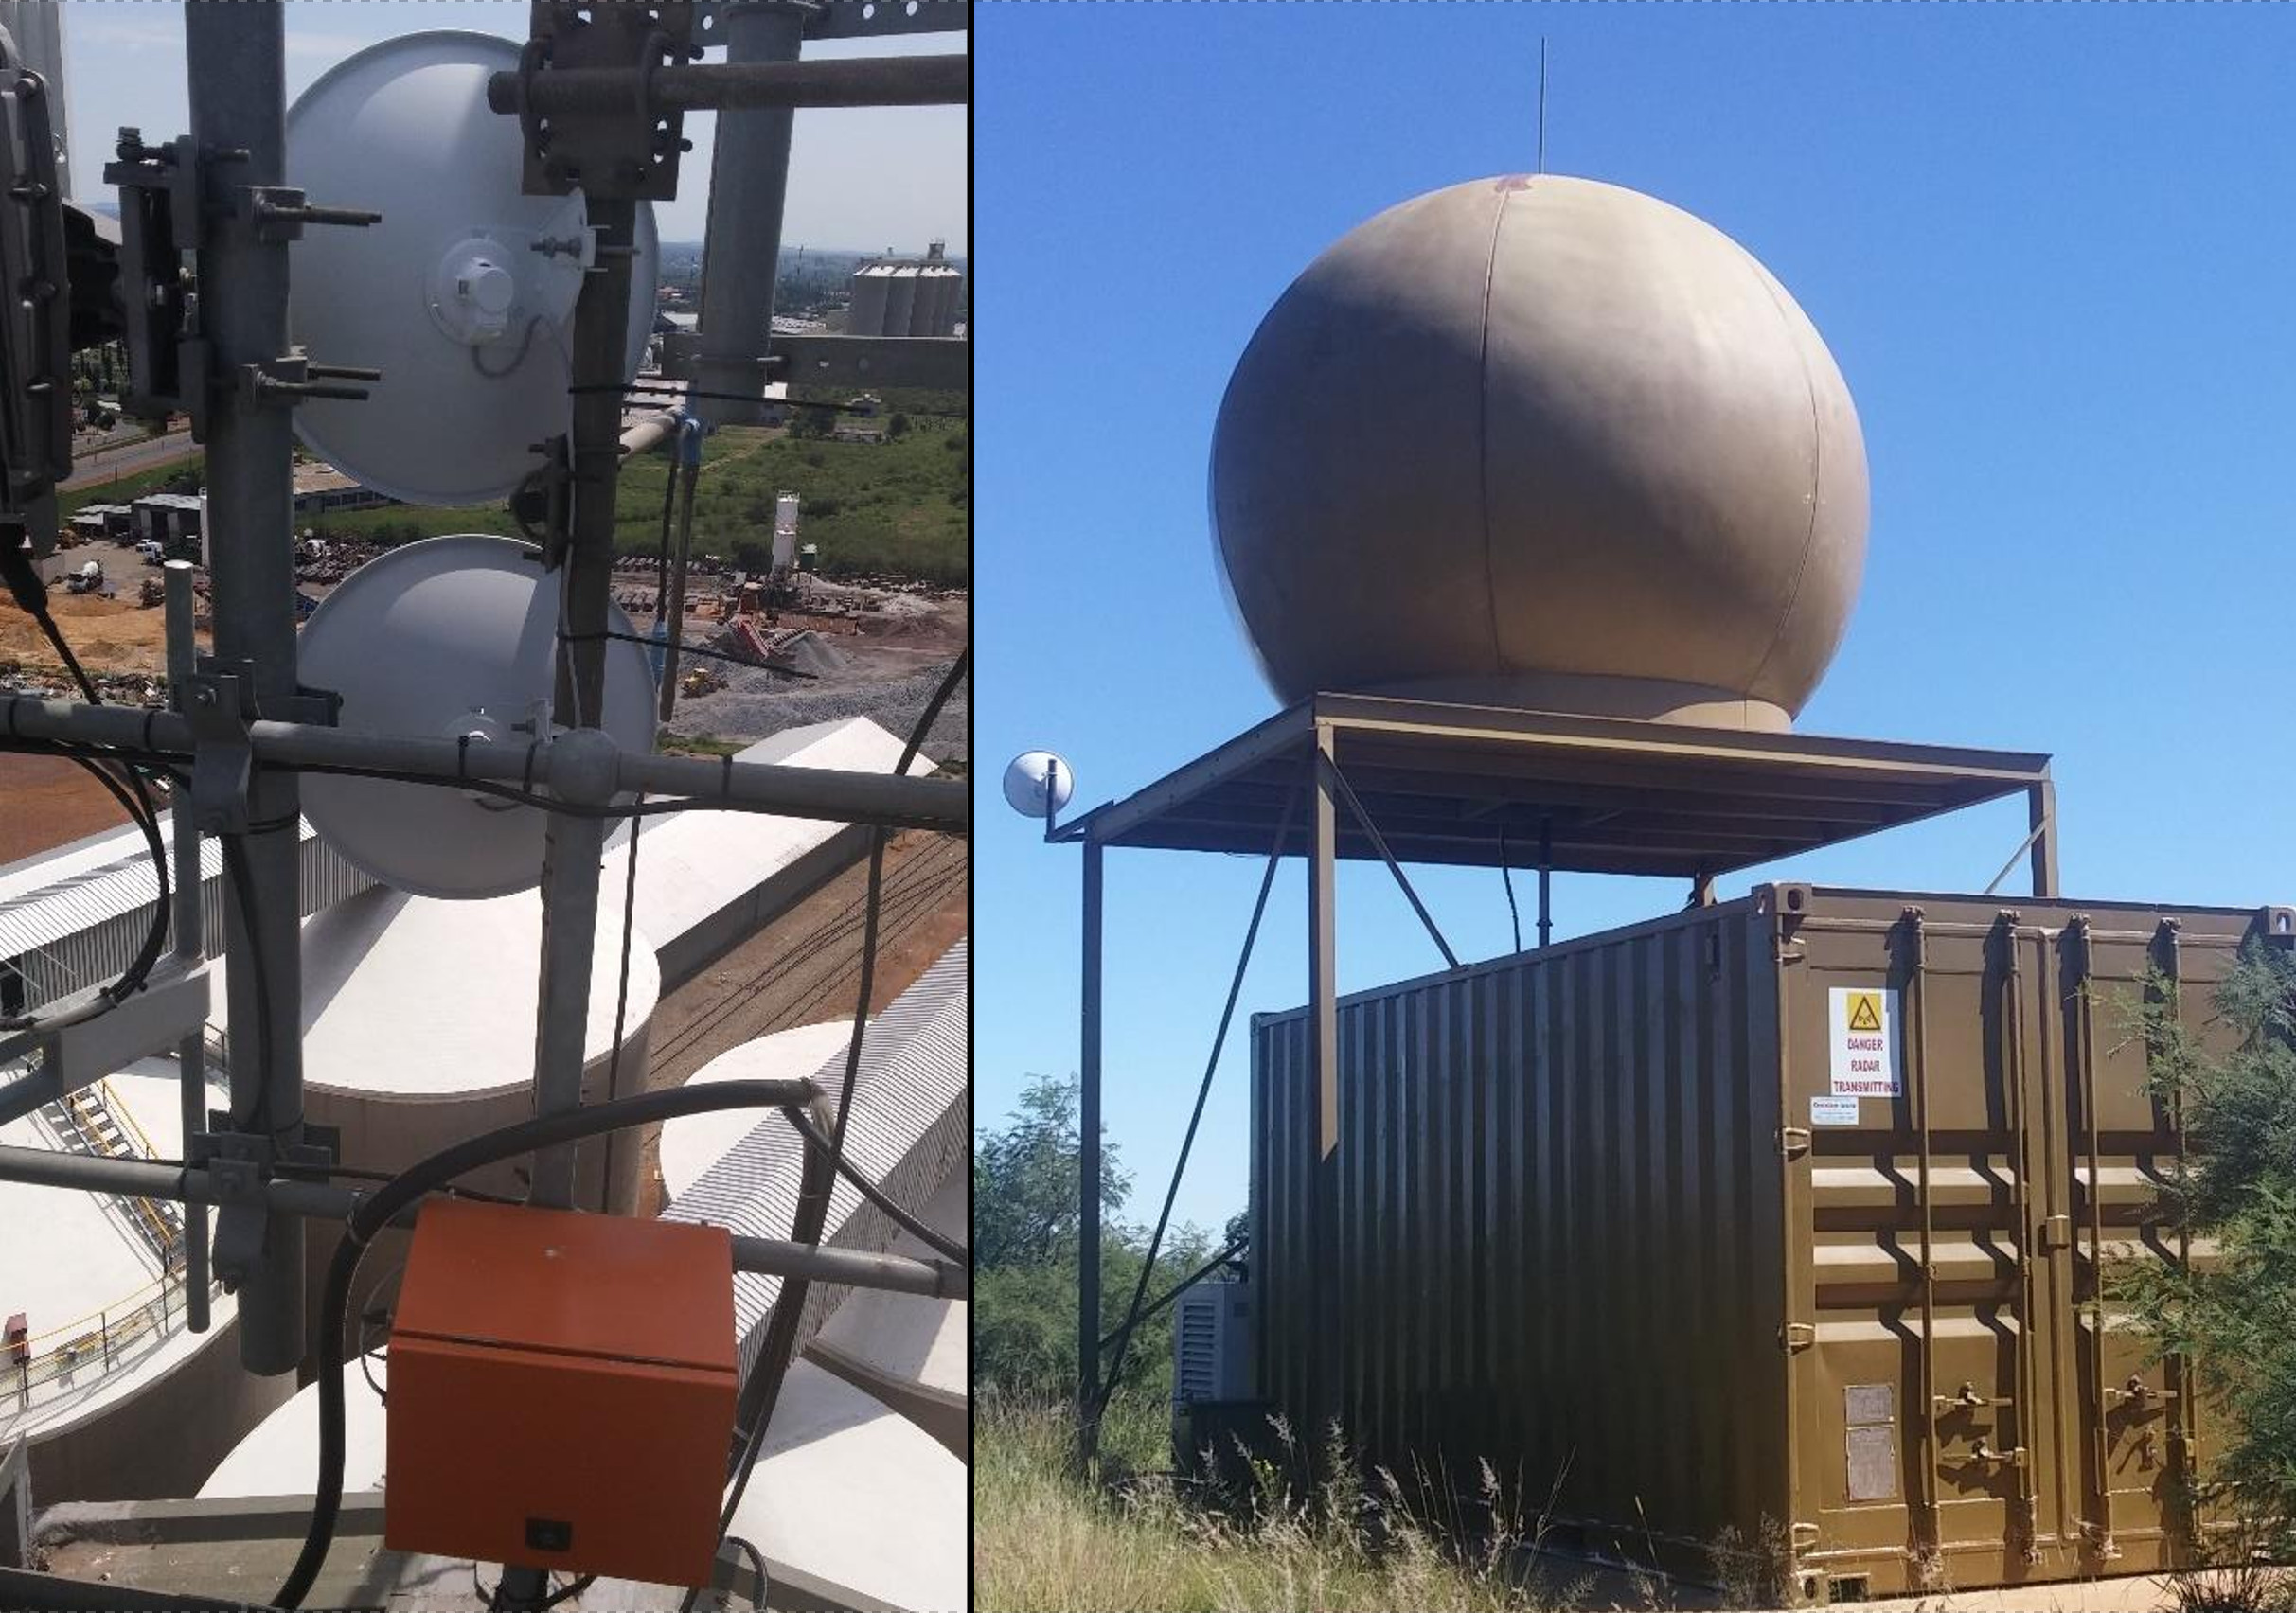
\includegraphics[width=\textwidth]{comlink1.jpg} \caption[The first
radio link established between the radar and the NWU.]{The first radio
link established between the radar and the NWU. The left photograph
shows the antennas on the silos and the right on the radar.}
\label{fig:link1}
\end{figure}

\begin{figure}
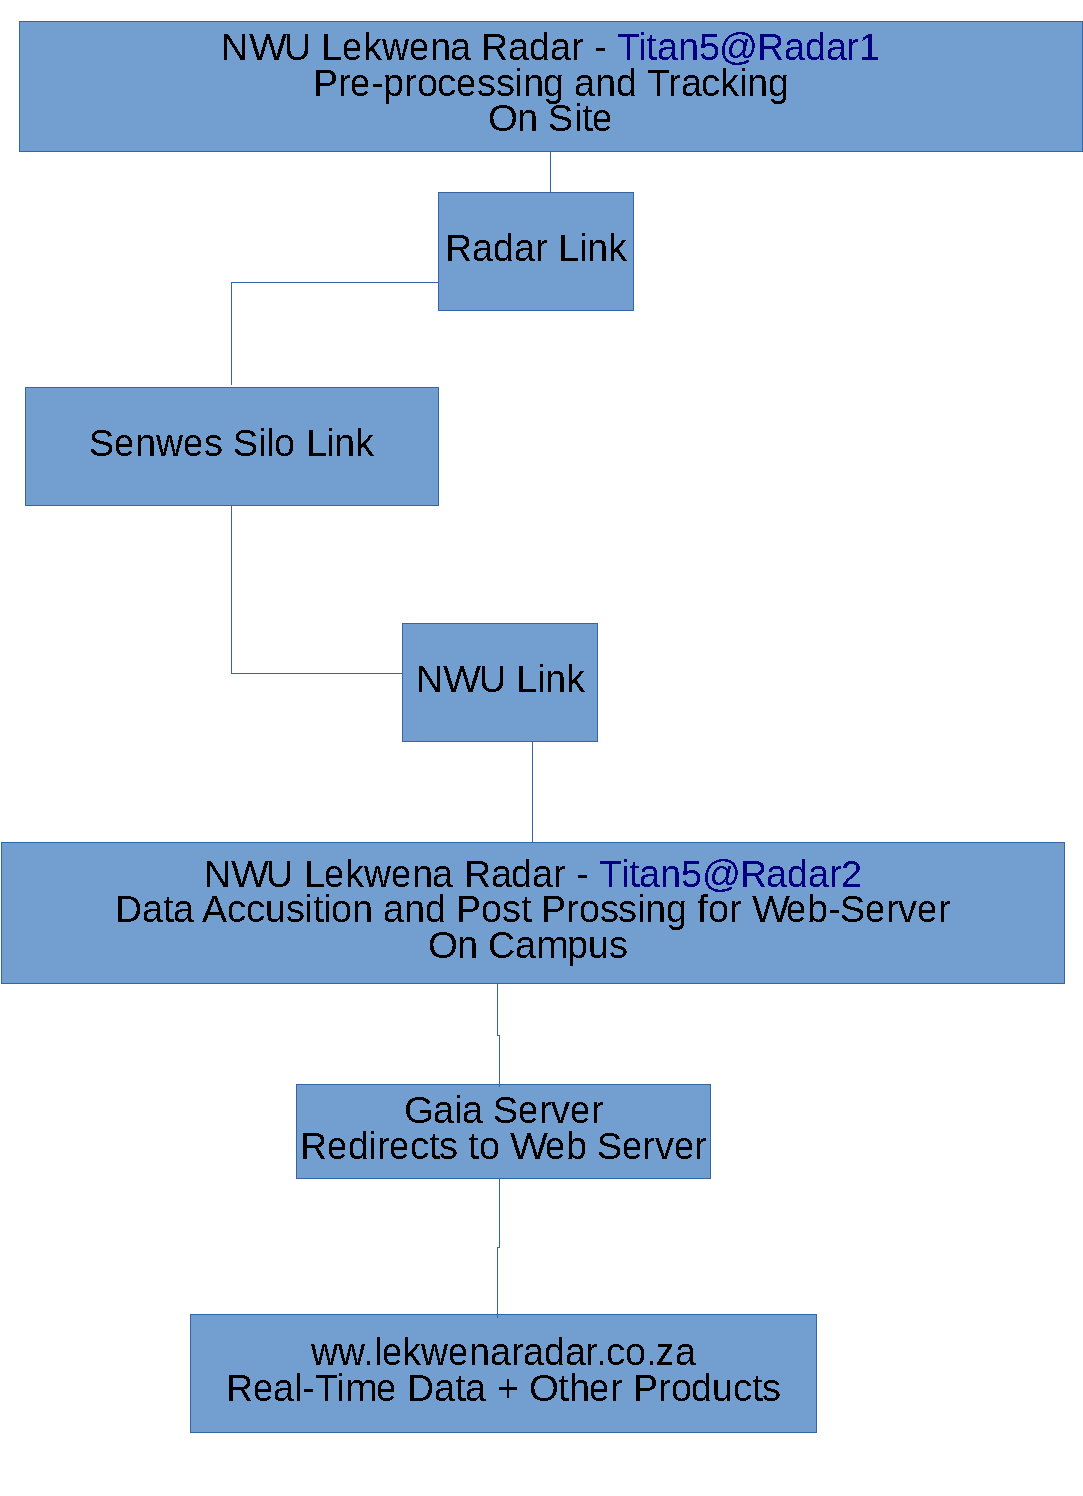
\includegraphics[width=\textwidth]{radarworkflow.pdf}
\caption[NWU CRG Radar Workflow]{In this diagram we see the workflow
of the NWU Lekwena radar from the radar sit to the web based service
driven by students. This is a simplified workflow and does not include
the technical aspects of the radar. To get data from the remote sit to
the university requires several key components. On site, there is a
server running Titan/RDAS software. Data is processed here initially.
This remote server is connected to the university through a wireless
link. The link sends data from the radar (link 1) to the silo's (link
2) located 16km away in Potchefstroom, the silo's was chosen due to
the height and direct line of sight with the radar, from the silo's
the next connection is to the university (link 3) where the data feeds
into radar2 server.} 
\label{fig:workflow}
\end{figure}

\section{A server to generate radar products}
\label{sec:radar2}

Data are transferred to the NWU in real-time using the titan
DsDistFile process of the \gls{lrose} software. A server (called
radar2) accepts the data that are being pushed by the radar server
(called radar1). Theis is a 8 core Intel i7 computer with \SI{2}{Tb}
disk space (Table~\ref{table:radar2}). It runs Ubuntu 16.04 and has
the latest version of the \gls{lrose} suite. It receives data in
real-time from the radar site (radar1) and then creates the static web
images. It then sends these images to the web server (gaia) and also
serves the raw radar data to the data server (bongani).

\begin{table}[!htbp]
  \caption[The technical specifications of the radar2 server.]{The technical specifications of the radar2 server.}
  \label{table:radar2}
  \begin{center}
\begin{tabular}{l l} 
\toprule
\bfseries Variable & \bfseries Property \\
\midrule
Processor & Intel(R) Core(TM) i7-4770K CPU @ 3.50GHz \\
Number of CPUs & 8 \\
CPU cash &8192 KB \\
Hard drive size & 2Tb \\
\bottomrule
\end{tabular}
  \end{center}
\end{table}

\section{A server to provide radar products for web sites}

The server that hosts the radar products is known as \textit{Gaia}. It
is a 4 Intel(R) Xeon(TM) CPU Linux Server (Table~\ref{table:gaia}). It
runs Ubuntu 16.04 LTS and is used as a basic web server to host the
static and dynamic radar images and text data files.

\begin{table}[!htbp]
  \caption[The technical specifications of the gaia server.]{The technical specifications of the gaia server.}
  \label{table:gaia}
  \begin{center}
\begin{tabular}{l l} 
\toprule
\bfseries Variable & \bfseries Property \\
\midrule
IP & http://143.160.8.22/ \\
Processor & Intel(R) Xeon(TM) CPU 3.00GHz \\
Number of CPUs & 4 \\
CPU cash & 2048 KB \\
Hard drive size & 80Gb \\
\bottomrule
\end{tabular}
  \end{center}
\end{table}

\section{A server to provide access to raw radar data}

Bongani is a 48 Intel(R) Xeon(R) CPU Linux Server
(Table~\ref{table:bongani}). Bongani was used in the past for
operational \gls{wrf} simulations. Currently Bongani is used as backup
solution for radar data and configuration files. It furthers runs an
instance of the \gls{lrose} software and can serve the raw data to any
other \gls{lrose} instance. It furthers provide a full service for the
data to be accessed over the Internet using the \textbf{Jazz}
application (see Section~\ref{sec:java}).

\begin{table}[!htbp]
  \caption[The technical specifications of Bongani.]{The technical specifications of Bongani.}
  \label{table:bongani}
  \begin{center}
\begin{tabular}{l l} 
\toprule
\bfseries Variable & \bfseries Property \\
\midrule
IP & 143.160.8.21 \\
Processor & Intel(R) Xeon(R) CPU E7540 @ 2.00GHz\\
Number of CPUs & 48 \\
CPU cash & 18432 KB \\
Hard drive size & 1Tb \\
\bottomrule
\end{tabular}
  \end{center}
\end{table}

\section{A Java application to view raw data in real-time}
\label{sec:java}

The \textbf{Jazz} java application is designed and supported by
\gls{ncar}. The application is described on its website:
\url{http://www.ral.ucar.edu/projects/jazz/}. It is designed as a
display system for MDV format data. It is therefore ideal to provide
quick access to the three dimentional raw data from the NWU Lekwena
radar (Figure~\ref{fig:jazz}). 

\begin{figure}[!htp]
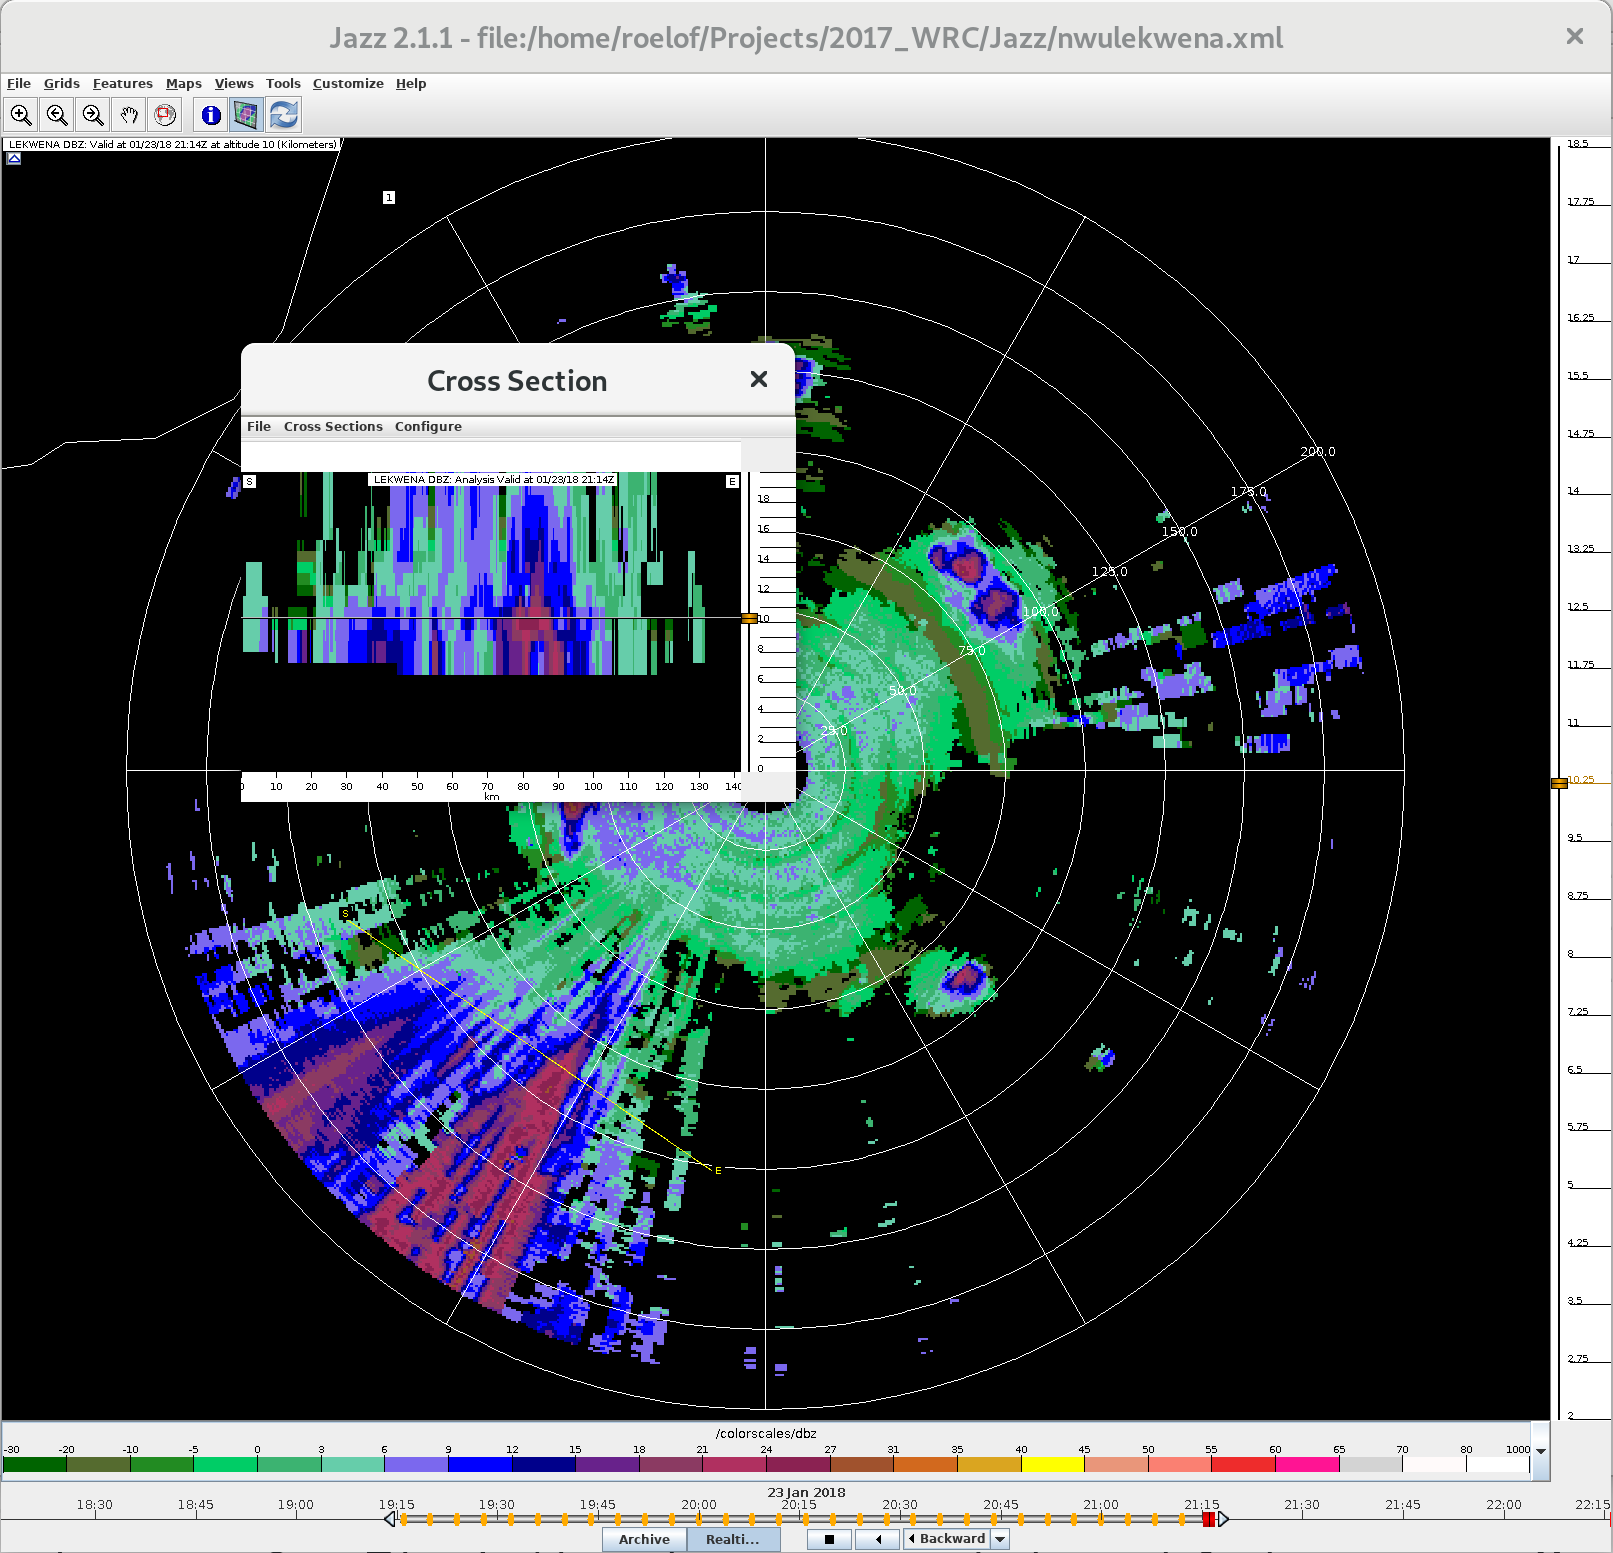
\includegraphics[width=\textwidth]{jazz-example2.png}
  \caption[The first radio link established between the radar and the
  NWU.]{The first radio link established between the radar and the
  NWU. The left photograph shows the antennas on the silos and the
  right on the radar.}
\label{fig:jazz}
\end{figure}

The most important parameters of the Jazz XML configuration file is
shown below:

\begin{verbatim}
<Jazz>
<Layer vis="on" type="MDV" name="LEKWENA DBZ"
location="mdvp:://143.160.8.21::mdv/radar/cartLaKwena"
field="DBZ" render="grid" 
colorscale="http://rap.ucar.edu/colorscales/dbz.colors"
menuGroup="nwu_short" />

<MenuGroup name="nwu_short" 
label="NWU short range" 
parentGroup="GRIDS_MENU" />

<Time mode="real-time" 
start="-45mins" 
end="+15mins" 
interval="4mins" 
update="5mins" 
timeZone="UTC" />

<Animation delay="75" dwell="3000" />

<Altitude dataDrivenProperties="true" default="2.4" />

<View projection="Flat" 
originLon="27.16770" originLat="-26.61886" 
rotation="0" />

<Window 
width="900" 
height="900" 
xOrigin="0" 
yOrigin="0" 
backgroundColor="black"/>

</Jazz>
\end{verbatim}

\section{A website to serve products in real-time}

A website was set up to serve products to stakeholders in real-time.
To use and deploy a website on the world wide wed a domain has to be
bought and registered from a third party. The current domain
registered is \url{www.lekwenaradar.co.za}. After a domain has been
registered a developer can build a website to the needs of the
organisation. The nature of the website and the living laboratory is
to empower and learn students and graduate students where assisted to
be directly involved in development of \url{www.lekwenaradar.co.za}.

A GitHub account was set up to facilitate version control of code
related to data analysis and visualization and to host the website. A
website is in development to improve the visibility of projects
completed, currently the \gls{gfs} models, satellite products and the
Lekwena radar output is showed on the website. The website aims to be
an simple, efficient platform to view and download data by scientists
from any research-entity without any concern for affiliation. Students
will be encouraged to learn interactively from the web platform by
viewing real-time weather, satellite and forecast data.

\url{www.lekwenaradar.co.za} was deployed using Jekyll and GitHub.
Jekyll allows websites to be build locally for testing before
deployment (Figure~\ref{fig:website}). A strategic decision was made
to keep the website static, this allows for a reliable and easily
manageable website trough GitHub. Students had to learn basic HTML and
Markdown to develop the website. A dedicated Linux server was acquired
for this purpose, the server is similar to radar2 server discussed
before (Section~\ref{sec:radar2}).

\begin{figure}[!htp]
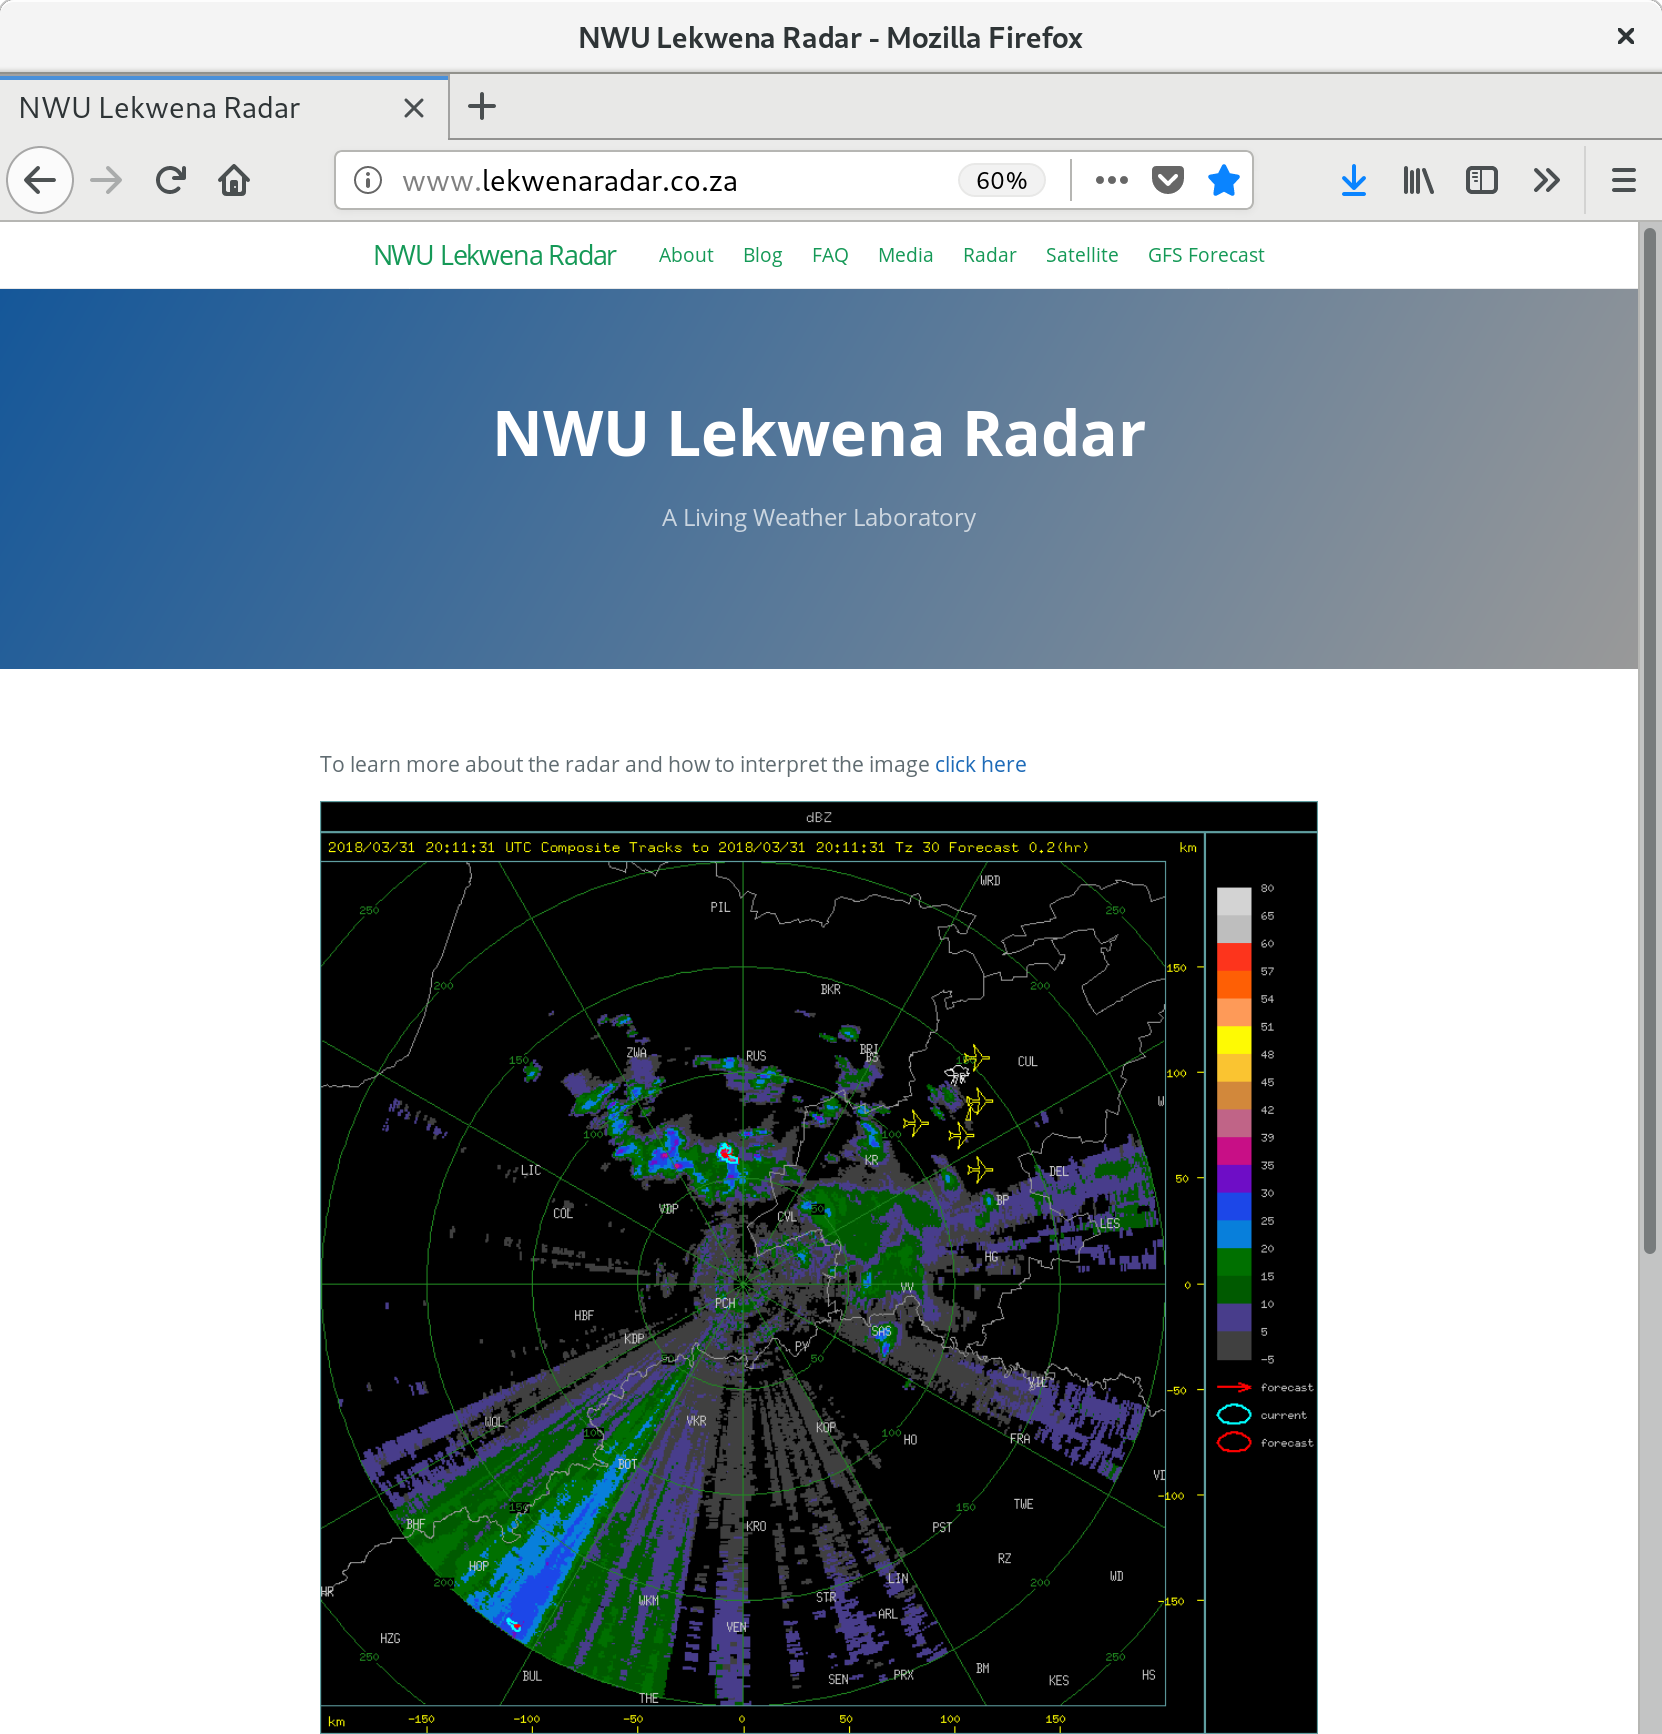
\includegraphics[width=\textwidth]{website1.png}
  \caption[The http://lekwenaradar.co.za website.]{The \url{http://lekwenaradar.co.za} website.}
 \label{fig:website}
\end{figure}

\chapter{Data management}

The focus of this project is to provide real-time data to stakehoders.
The ammount of data generated is significant. Including data products
can reach up to \SI{1}{Gb} per day. The \gls{crg} are therefore being
forced to implement a solid data management plan in order to ensure
the availability and reliability of data. 

The \gls{crg} currently collects data from a variety of sources for
research purposes. An overview of the work flow is shown in
Figure~\ref{fig:workflow}. The \gls{nwu} Lekwena C Band radar is in
the process of becoming fully operational while the Mooi River Rain
Gauge network has been deployed and is up and running. Along with
these operational instruments, the \gls{nwu} actively runs it's own
\gls{gfs} and \gls{wrf} models. All the data is used by students and
researchers to understand various land system interaction and
processes. The following chapter describes the current scientific
tools and data management systems in use by the \gls{crg}.

\section{Reanalysis Data} The \gls{crg} currently has several servers
running on the \gls{nwu} network (See Chapter~\ref{chap:real-time}).
Currently Bongani is used as backup solution for radar data and
configuration files. The second local server is the \textit{Titan5}
dedicated radar host. The Titan network links to \textit{Gaia} used as
a web host to provide the radar data to the public. The \gls{crg} also
has access to the \gls{nwu-hpc}, a 32 core Linux server maintained by
the \gls{nwu}, the \gls{nwu-hpc} is used for running low resolution
weather simulations using \gls{wrf} and testing compiling and run time
options for various climate models.  The \gls{crg} also has access to
the \gls{ncar} Yellowstone supercomputer for high resolution modeling.

\section{Radar Data} The radar data is stored on both the radar1 and
radar2 servers. It is futher transferred to an onine Dropbox cloud
storage account. All students have access to a allocated Dropbox
account where they are required to store all data collected as part of
their research. Dropbox has been the best cloud solution as it has
Linux, Windows and Mac clients. Data stored and managed trough this
cloud solution has been a key part in case of system failure and
theft.

\section{Satellite Data} Satellite data for the study area are being
served through the project website. These products will be further
integrated into the project website over the next year.

\begin{figure}
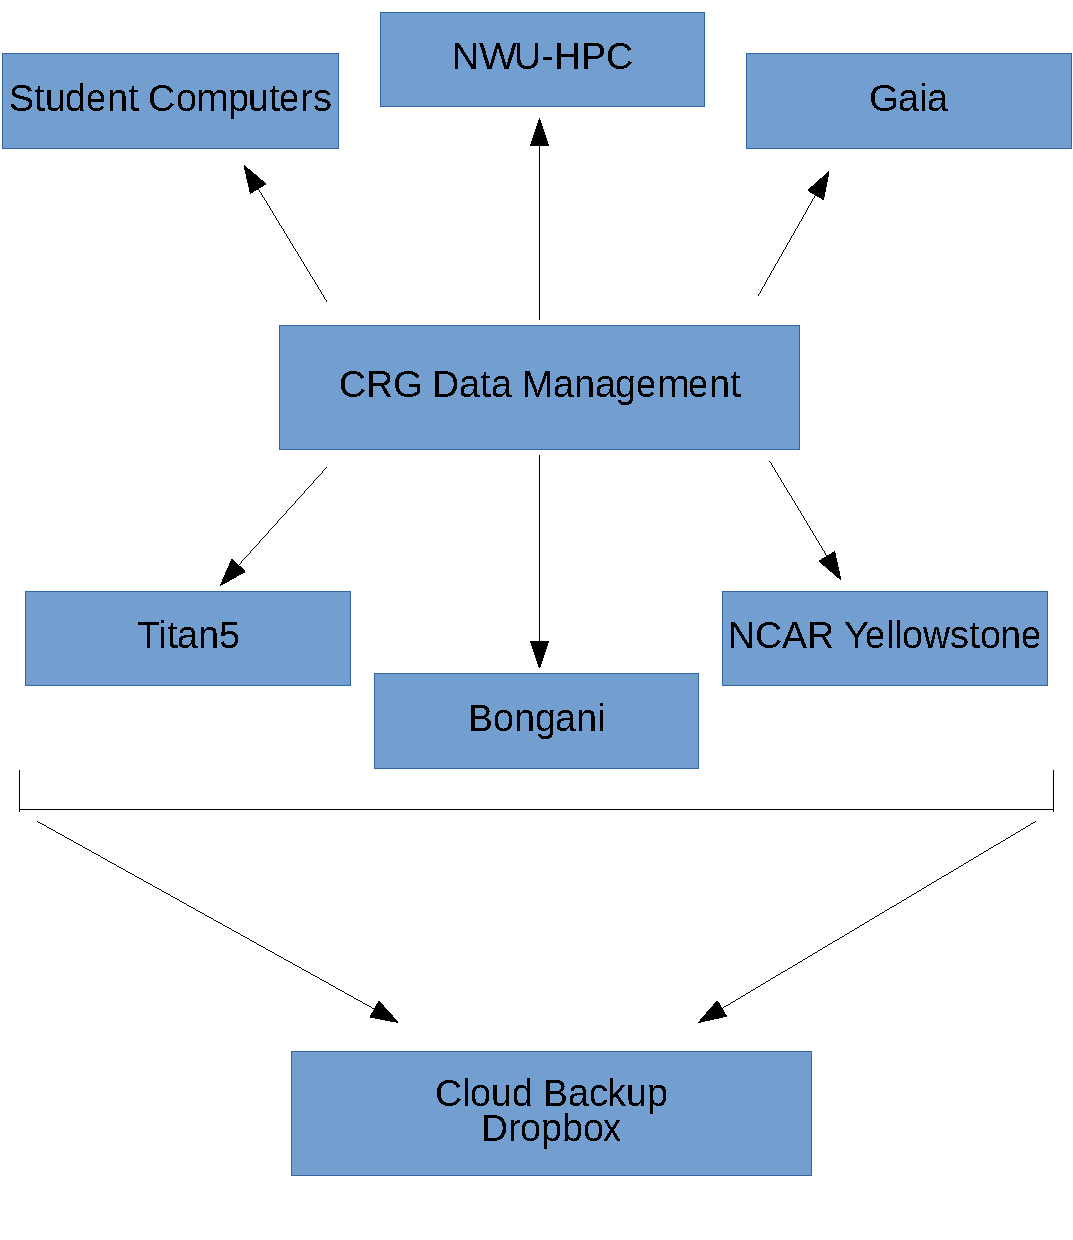
\includegraphics[width=\textwidth]{ComputerSolutions.pdf}
\caption[NWU CRG Data Management Setup]{The diagram indicates the
current work flow related to the NWU CRG data management strategy. The
data management starts on local computers assigned to all students,
technicians and researchers. The \gls{crg} has several local servers
on which data is then stored and managed for access across the project
team, this includes \textit{bongani} and Drobox. The radar data
collected feeds directly to two dedicated servers - \textit{titan5}
and \textit{gaia}. Gaia also hosts the radar visualization that is
shown on the websites.}
\label{fig:data_workflow}
\end{figure}

\section{Observational Data}

A network of rain gauges are being fitted with modems to provide
real-time access to rainfall and other weather parameters. These
datasets are also served through the website.

\section{Data visualization}
Visualizing data products plays an important role for user friendly interpretation
and also spatial temporal representation of data. Currently GFS model data is
visualized every day to provide an 48 hour forecast to users whom access the
www.lekwenaradar.com. Further development is in place to provide a real-time
analysis of rainfall trends data in the Mooi River catchment, this is dependant upon
the deployment of LORA and Foxnet networks. The
radar products are continually being improved for the web interface.

\section{Cloud Storage}
For data backup a 2 terabyte Dropbox cloud solution was acquired.
Dropbox is only used as for backup of data in case of server failure.
All students have access to a allocated Dropbox account where they are
required to store all data collected as part of their research.
Dropbox has been the best cloud solution as it has Linux, Windows and
Mac clients. Data stored and managed trough this cloud solution has
been a key part in case of system failure and theft.

\section{Password Management}
All students and researchers are assigned a LastPass account. LastPass
is a password manager, users can generate strong random passwords
that's encrypted through LastPass. Passwords are also randomized
between accounts to avoid password reuse and avoid security breaches.
LastPass also allows for storage of ssh keys to access servers.

\section{Connecting CRG projects}
Figure \ref{fig:data} provides an indication of the holistic nature
related to the \gls{crg} research.  The major focuses groups include
the real-time weather and climatology initiatives while the second
major focus is related to air pollution studies. These two fields are
not seen as independent pillars within the research group, but instead
as one major end goal. These two fields are examined to quantitatively
understand the effects that each may have on the other.  The main
motivation behind the research done at the \gls{crg} is to improve the
lives of the local communities who suffer the most from these impacts
related to climate change and health problems from pollution.

\begin{figure}[htp]
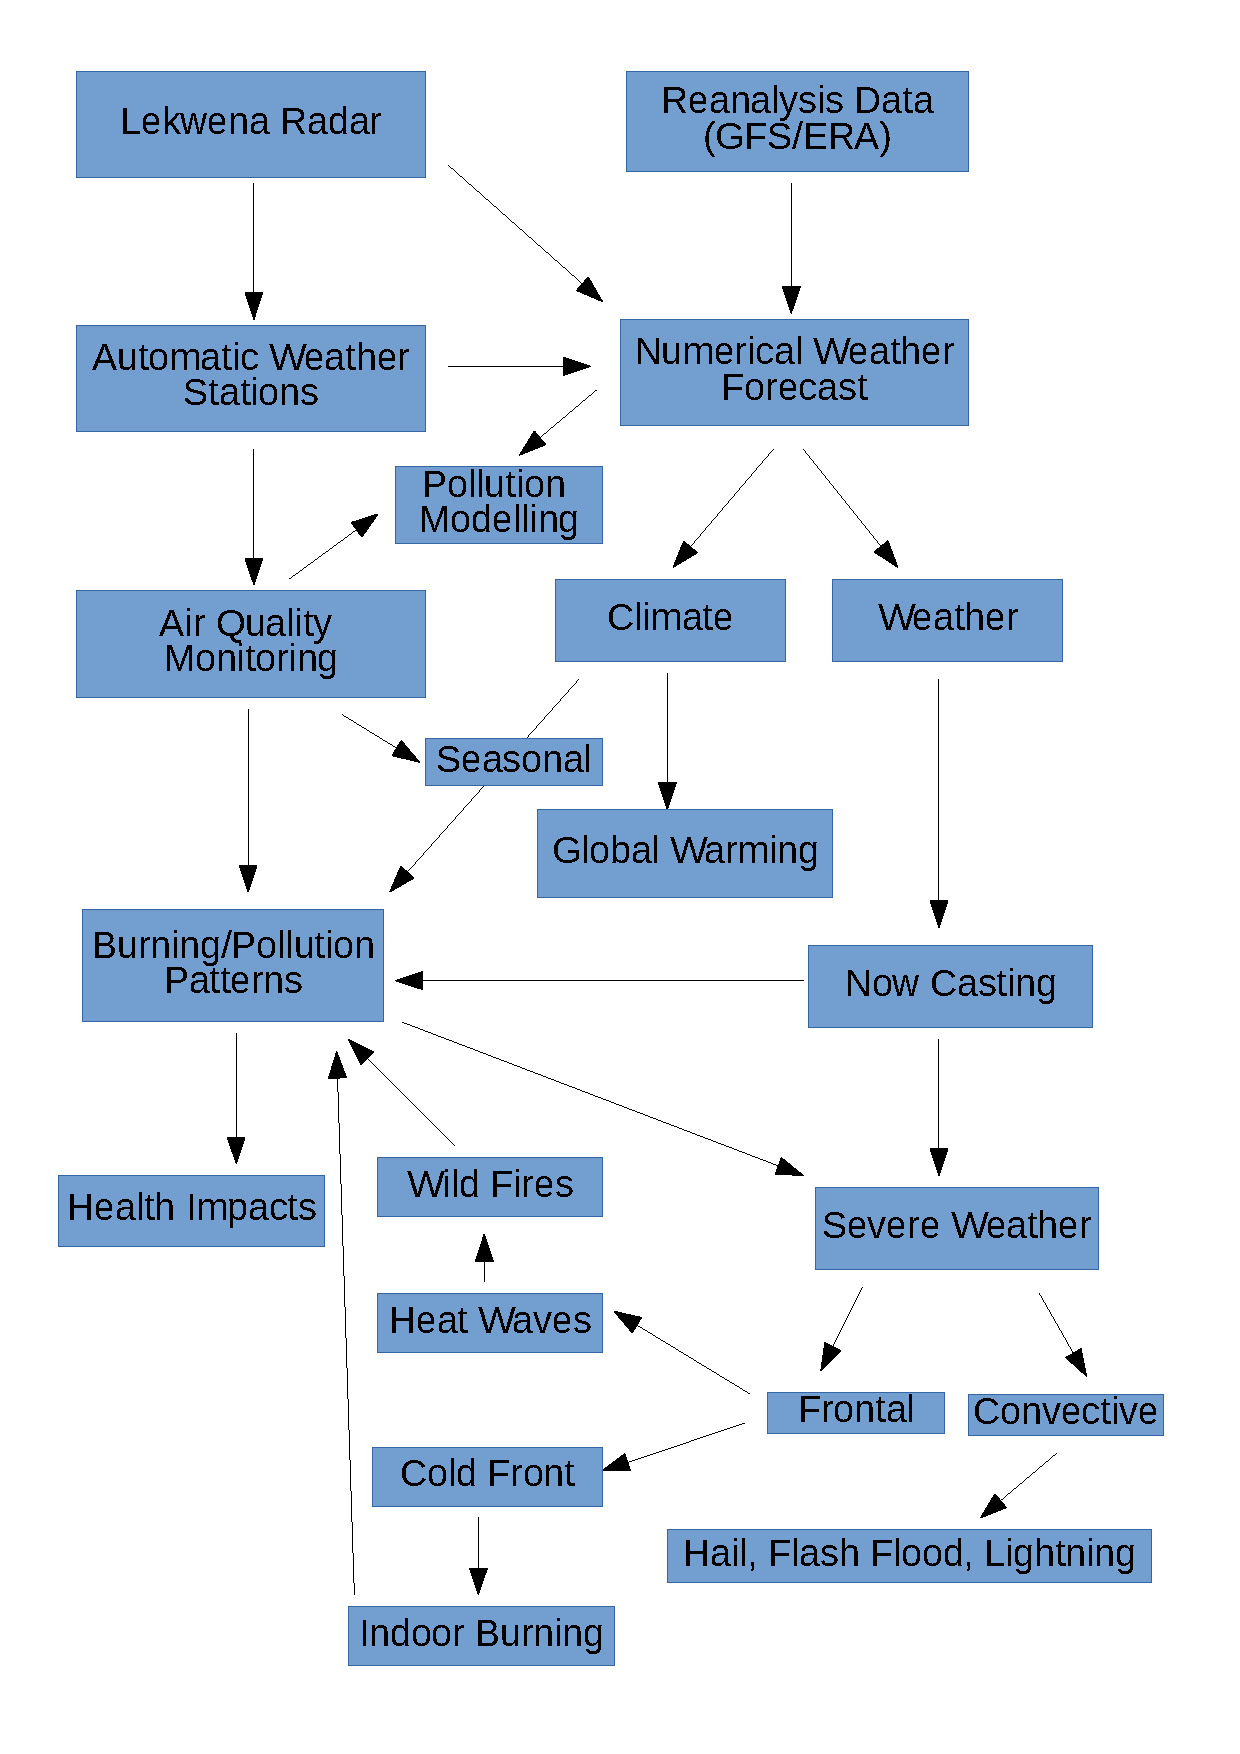
\includegraphics[width=\textwidth]{intersectional.pdf}
\caption[NWU CRG Resrearch Intersections]{The diagram indicates how
the different sources of data the CRG works with connects to each
other. All these data sources add up to a significant of amount of
data collected on a daily basis. Without a structured plan and
management system data could get lost, mismanaged or never analysed at
all. One of the main goals of the CRG is to create a sustainable data
management system that other organisations can use and build upon. The
CRG also strives to create an open access database where researchers
and students can access data free of charge} \label{fig:data}
\end{figure}

\chapter{Conclusions}

Progress have been made towards the stated objectives. Seven students
are directly involved in the project, with a further 10 honours
students being exposed to the science and technology through workshops
and hands on experience in 2017 and 6 honours students in 2018. One of
the 2017 students have joined the project and two of the 2018 honours
students are doing their research projects on this project.

This report focus on the work performed to ensure real-time access to
the data generated during this project. The overall aim of this
project is to build national capacity to ensure the sustainable use of
the national observation weather infrastructure. We believe that a
facility that provide real-time access to universities and other
stakeholders can play an important role in bringing together a
community to foster and enhance capacity building around the
observation of weather in South Africa.

The observational infrastructure of this project includes the NWU
Lekwena radar, a network of rain gauges and a few automatic weather
stations. As part of this component, a microwave link was set up
network the radar with the \gls{nwu}. Derived products are served on a
website (\url{http://www.lekwenaradar.co.za}). Real-time access to the
full four dimentional radar dataset are provided by a \gls{lrose}
server that makes it possible for anyone to explore the data using the
Jazz Java application. Stakeholders can also be provided with the data
in real-time using an \gls{lrose} server. All other data are available
through the project website. It is the first time in South Africa that
access to these datasets are provided at this level.

Efforts continue to increase the reliability of the network to ensure
continues operation. Interference from unlicensed WiFi networks
remains a problem and deteriorates the rainfall products from the
network. Talks with the Independent Communications Authority of South
Africa (ICASA) continue to find a solution to this problem. The
loggers are being deployed in the rain gauge network. The next report
will document these and other work performed on the project. A report
detaling the progress on the other objectives are the next
deliverable. It should be complete by the middle of April 2018.

%\addcontentsline{toc}{chapter}{Appendix A: Calibration documents}
%\includepdf[pages={-}]{Bethlehem-calibration.pdf}

\begin{spacing}{0.3}
\linespread{0.8} \normalsize
\bibliography{library}
\end{spacing}

\end{document}
